%&pdflatex

\documentclass[12pt,letter]{article}
%%%%%%%%%%%%%%%%%%%%%%%%%%%%%%%%%%%%%%%%%%%%%%%%%%%%%%%%%%%%%%%%%%%%%%%%%%%%%%%%
\usepackage{booktabs, caption, subcaption, float}
\usepackage[latin1]{inputenc}
\usepackage{longtable}
\usepackage{graphics}
\usepackage{geometry}
\usepackage{graphicx}
\usepackage{amsfonts, amssymb, amsmath}
\usepackage{natbib, multibib}
\usepackage{theorem}
\usepackage{setspace}
\usepackage[normalem]{ulem}
\usepackage{caption}
\usepackage{tabularx}
\usepackage{epstopdf}
\usepackage{rotating}
\usepackage{placeins}
\usepackage[makeroom]{cancel}
\usepackage{varioref}
\usepackage{hyperref}

\setcounter{MaxMatrixCols}{10}
% TCIDATA{OutputFilter=Latex.dll} TCIDATA{Version=5.50.0.2960}
% TCIDATA{<META NAME="SaveForMode" CONTENT="1">}
% TCIDATA{BibliographyScheme=BibTeX} TCIDATA{LastRevised=Monday, May
% 11, 2015 19:08:26} TCIDATA{<META NAME="GraphicsSave" CONTENT="32">}

\theoremstyle{break} \theorembodyfont{\normalfont\itshape}
\newtheorem{thm}{Theorem}
\theoremstyle{break}
\theorembodyfont{\normalfont\itshape}
\newtheorem{corrollary}{Corollary} \theoremstyle{break}
\theorembodyfont{\normalfont\itshape} \newtheorem{prop}{Proposition}
\theoremstyle{break} \theorembodyfont{\normalfont\itshape}
\newtheorem{lemma}{Lemma} \theoremstyle{break}
\theorembodyfont{\normalfont\itshape} \newtheorem{algm}{Algorithm}
\theoremstyle{break} \theorembodyfont{\normalfont\itshape}
\newtheorem{definition}{Definition} \theoremstyle{break}
\theorembodyfont{\normalfont\itshape}
\newtheorem{condition}{Condition} \theoremstyle{break}
\theorembodyfont{\normalfont\itshape}

\renewcommand{\baselinestretch}{1.5}
\setlength{\hoffset}{-0.4in}
\setlength{\textwidth}{6.8in}
\setlength{\textheight}{9.3in}
\setlength{\topmargin}{-0.5in}



\begin{document}

\author{Tarek A. Hassan\thanks{\textbf{Boston University}, NBER, and
    CEPR; Postal Address: 270 Bay State Road, Boston, MA 02215, USA;
    E-mail: thassan@bu.edu.} \and
  Tony Zhang\thanks{\textbf{%
      Boston University, Questrom School of Business}; Postal Address:
    595 Commonwealth Avenue, Boston, MA 02215, USA; E-mail:
    tzhang0@bu.edu.} }

\title{The Economics of Currency Risk Premia\thanks{}}

\date{ \bigskip July 2020}

\maketitle

% +Title

\thispagestyle{empty}


\vspace{-0.7cm}


\setstretch{1.0}



\begin{abstract}
  This article reviews the literature on currency risk with a focus on
  its macroeconomic origins and implications. A growing body of
  evidence shows that countries with safer currencies enjoy
  persistently lower interest rates, a lower required return to
  capital, and accumulate relatively more capital than countries
  international investors perceive as risky. While earlier research
  has focused mainly on the role of currency risk in generating
  violations of uncovered interest parity and other financial
  anomalies, more recent evidence also points to important
  implications for the allocation of capital across countries, the
  efficacy of exchange rate stabilization policies, the sustainability
  of trade deficits, and the spill-over of shocks across borders.
\end{abstract}


\bigskip

\bigskip {\noindent \textbf{JEL classification:} }

{\noindent \textbf{Keywords:} }

\pagebreak

\setstretch{1.4} \setcounter{page}{1}


\section{Introduction}


A key tenet in economics is that the degree to which firms should be
willing to invest in a given project depends crucially on the required
rate of return to capital: a price-taking firm should install just
enough capital so that the marginal product of capital, $MPK_i$, equals
the required rate of return to capital,$r_i$, 
\begin{equation}
    MPK_i=\underbrace{r^f+RP_i}_{r_i}.
    \label{eq_one}
\end{equation} 
This equation is the point of departure for many classic questions in economics. Students of asset
pricing are taught that a firm's $r_i$ has two components; a risk-free
part, $r^f$, and a risk-premium, $RP_i$, that depends on the firm's
risk characteristics. One of the classic puzzles in asset pricing is
why $RP_i$ is so large relative to $r^f$ (the equity premium puzzle).
Monetary economists are interested in the Federal Reserve's power to
manipulate $r^f$, while students of economic growth often take
differences in $MPK_i$ as a measure of inefficiencies in the
allocation of capital across countries, sectors, and firms.

In this article we argue that recent insights from the study of
currency risk premia have important lessons for how we should think
about equation (\ref{eq_one}), and by extension, for its key
applications in asset pricing, macroeconomics, and economic growth.
The simplest, and perhaps and most important, of these lessons is that
countries differ dramatically in their risk-free interest rates. These
differences in risk-free interest rates are large (on the same order
of magnitude as the equity premium puzzle), appear to be highly
persistent over time (lasting for decades rather than years), and
cannot be explained by predictable depreciations, government default,
or differences in inflation rates. Instead, these differences in
interest rates appear intimately linked to the risk characteristics of
the country's exchange rate, and to its exchange rate regime.

\begin{figure}
    \centering
    \caption{Risk-free Interest Rates}
    \includegraphics[width=0.7\textwidth]{Exhibits/Figure_FP12M_JPYNZD.pdf}
    \label{fig:fp}
\end{figure}
Figure \ref{fig:fp} shows the difference in the risk-free interest rates of the
New Zealand Dollar and the Japanese Yen as an example (we will discuss
below how one can measure such risk-free rates and compare them across
countries). The Figure shows that the New Zealand dollar had a higher
risk-free rate than the Japanese Yen in \textit{every} month between
January 1996 and December 2018. On average, this difference was about 
4.39pp on an annualized basis. When we adjust for movements in exchange rates over
the period, the difference in returns on the two countries currencies
is XXpp -- meaning that a US investors who borrowed in Yen and lent in
New Zealand Dollars on average made a return of XX percent over this
period. (For comparison, the equity premium on US stocks was about
XXpp during the same period.)

We now know that such highly persistent differences in interest rates,
similar to those between New Zealand and Japan, are common in the
data, even among developed economies. These large differences in
interest rates do not appear to be equalizing over
time and translate into large differences in returns investors can
earn when investing in these currencies.

Why would $r^f$ differ permanently across countries? The emerging
consensus in the literature is that the most likely explanation are
currency risk premia -- the idea that some currencies are safer
investments than others. 

A useful way of thinking about this problem
is to take the perspective of a retail investor in a third country, say in Hong Kong.
As is common in many countries, Hong Kong-based banks regularly offer savings accounts denominated in multiple currencies, so that our fictitious investor might have the option to invest in yen at a deposit rate of 0.1\% or in New Zealand Dollars at a rate of 3.0\%. How might she decide between these two options? Since both accounts are with the same bank, any likelihood of sovereign default is irrelevant. Similarly, our Hong-Kong based investor does not care about inflation in these two faraway countries. Instead, the only relevant factors for her choice between these two investment is the difference in interest rates and the stochastic behavior of the yen-to New Zealand dollar exchange rate. 

Because changes in exchange rates are largely unpredictable over short horizons, our investor should not expect either currency to depreciate over the coming year, leaving only one relevant consideration: covariance. Which of the two currencies does our investor trust to retain value in a possible recession or crisis? Intuitively, she might think that Japanese yen are a safer bet -- and she would be right. Along with a number of other so called ``safe-haven currencies,'' the Japanese yen tends to appreciate relative to the New Zealand dollar during large international recessions and crises. If yen are a safer store of value, it might make sense to accept a lower deposit rate. That is, international investors might be willing to lend at lower rates in currencies they expect to retain value when times are bad. 

As it turns out, this simple intuition has a lot of support in the
data from international bond and derivatives markets. For example, a seminal paper by \citet{LustigVerdelhan2007}
shows that currencies with low interest rates on tend to appreciate
when US consumption growth is low, and depreciate when US consumption
growth is high. That is, there is direct evidence that currencies with
low interest rates appreciate when times are ``bad'', making them a
safer store of value for investors.

In addition to this empirical evidence, the theoretical work on
currency risk has identified compelling theoretical reasons to expect
the emergence of safe-haven currencies and long-lasting differences in
interest rates. In a nutshell, currency risk premia arise naturally in
a wide range of international macro models. For example, \citet{Hassan2013}
shows that simply allowing for some economies to be larger than others
within a standard international real business cycle model is
sufficient to generate long-term differences in interest rates between
countries, because the currencies of larger countries tend to
appreciate when world-wide output is low. That is, even within the
most canonical, frictionless, international macro models currency
risk premia tend to arise naturally in equilibrium. Other authors have
similarly pointed to the emergence of currency premia in models with
intermediary capital constraints, trade costs, and differences in
resource endowments, among others.

A major difficulty this literature shares with a broader literature in
asset pricing is that models with conventional preferences tend to
produce risk premia that are quantitatively small. That is, although a
number of papers have identified compelling reasons why, for example,
the interest rate in Japan should be lower than that in New Zealand,
most of these models suggest that it should be lower by something on
the order of 0.04pp rather than the 4.23pp we measure in the data. In
this sense, the literature is running into a quantitative ``interest
differential puzzle,'' which is in some ways analogous to the equity
premium puzzle. Both puzzles fundamentally struggle with the
prediction of models with standard preferences that risk premia should
be small given the relatively small aggregate variation in consumption
growth we measure in the data. Quantitative research on currency risk
is thus a major area for future research.

We survey the rapidly growing empirical and theoretical literature on
currency risk premia in detail in sections XX and XX. Because the
initial focus of this literature was mainly on resolving asset pricing
anomalies, many of its key papers tend to use technical finance language.
For this reason we attempted to keep this review as non-technical as
possible, focusing as much as possible on the underlying economics.

Although the literature on currency risk premia has proliferated in
recent years, it has perhaps been less successful at making clear the
relevance of its findings beyond the financial context, a gap we hope to
partially fill with this article.

Perhaps the most immediate implication of currency premia for the real
economy is for capital accumulation: If countries differ persistently
in $r^f$, then those with higher interest rates have a persistently
higher cost of capital and thus, according to (\ref{eq_one}) should
produce with relatively less capital. Returning to our example from
Figure \ref{fig:fp}, it turns out that indeed the capital-to-output ratio K/Y in
New Zealand is 22 percent lower than in Japan, suggesting that,
indeed, the marginal product of capital is larger in New Zealand than
it is in Japan. More generally, countries with persistently higher
interest rates appear to have higher marginal products of capital in
the long-run. This simple insight has direct implications for several
strands of the macroeconomic literature.

The first is for the so-called Lucas-puzzle \citep{Lucas1988}, which
posits that, over long periods of time, capital-to-output ratios do not appear to be equalizing across countries, and in particular, not enough capital appears to be flowing to developing nations to equalize the marginal product of capital. If indeed some currencies are permanently riskier than others, then currency risk is one possible factor preventing such equalization.

A second, related, implication is for a large literature that focuses on assessing the efficiency of the allocation of capital across countries \citep{HallJones1997, CaselliFeyrer2007}. A basic assumption in this literature is that $r^f$ is equalized across countries, so that systematic deviations from this required rates can (partially) be attributed to inefficiencies. However, if there are fundamental (efficient) reasons for $r^f$ to differ due to differing currency (and country) risk characteristics, some of these calculations will have to be modified.

Third, an active literature in international finance has studied the propensity of firms and countries to borrow in foreign currency \citep{DuSchreger2016, KalemliOzcanetal2019}. If lending in a low-interest-rate currency is safer than lending in a high-interest-rate currency, then the opposite is true for borrowing. That is, firms that borrow in dollar, yen or another safe-haven currency may be loading up on systematic risk -- a price they pay for enjoying lower rates.

Aside from issues surrounding capital accumulation and investment, long-lasting differences in interest rates across countries may also change how we think about two major XXX. The United States and a number of other countries is running a persistent current account deficit, the sustainability of which depends crucially on its ability to borrow cheaply in international markets \citep{GourinchasRey2007}. If there are fundamental economic reasons why the US dollar is a safer currency than many others, then lower US interest rates are here to stay, potentially enabling the United States to sustain trade and current account deficits in perpetuity.

If there is indeed something to this story, it changes how we think
about central issues in macro.

 4) Exchange rate regimes and risk 5)
Dynamics, capital flows and risk


\section{Risk-free Interest Rates, Exchange Rates, and Currency
  returns}

Measuring Risk-free interest rates using CIP.



Hassan and Mano facts, Violations of UIP, Fama 84



\section{Interest Rate Differentials as Differences in Risk Premia}

\begin{figure}
    \centering
    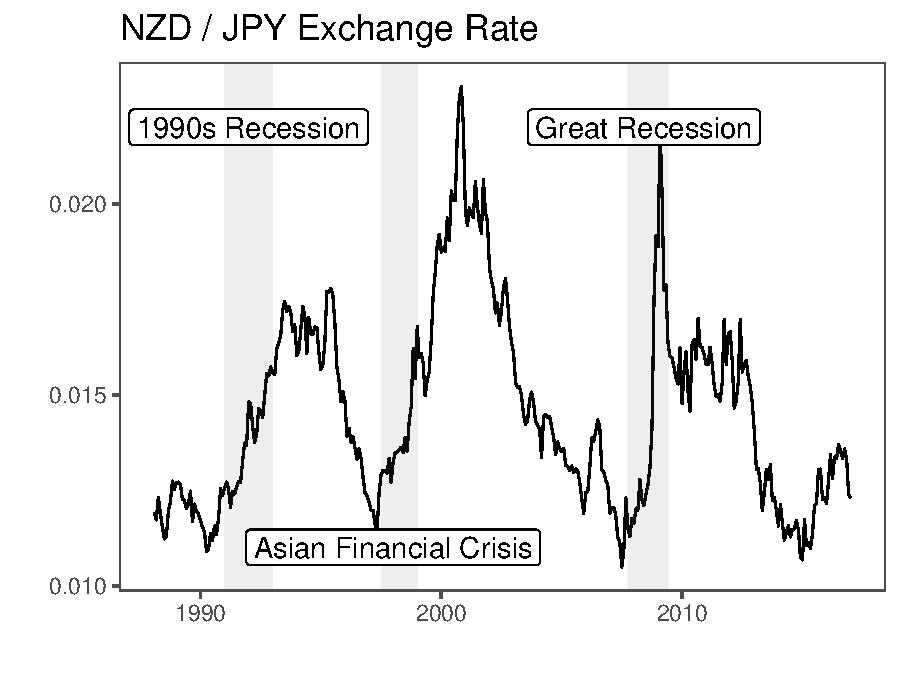
\includegraphics[width=0.7\textwidth]{Exhibits/Figure_FX_JPYNZD.pdf}
    \label{fig:spot}
\end{figure}
Continuing with our example from Figure \ref{fig:fp}, Figure \ref{fig:spot} plots the New
Zealand dollar - Japanese yen exchange rate in terms of dollars per
yen. An increase in the exchange rate indicates yen appreciation.
The shaded areas highlight three distinct periods of global economic
turmoil: The early 1990s recession (1990 - 1994), the Asian financial
crisis (1997 - 1998), and the Great Recession (2007 - 2009). In each of these periods of turmoil, the yen appreciated markedly against the New Zealand Dollar. If these appreciations during periods of economic
turmoil are part of a broader pattern, investors should naturally consider the Japanese yen the safer
currency. Hence, the lower returns earned on Japanese yen investments 
may be a result of the yen's usefulness as a hedge against bad times. 
On the other hand, we should expect investing in the New Zealand dollar 
earns higher returns, because the New Zealand dollar provides none of 
the hedging benefits of the Japanese yen and is therefore a riskier 
currency for global investors.

\subsection{Reduced-form Evidence}

In a seminal paper, \citet{LustigVerdelhan2007} provided  the first systematic evidence 
that low-interest-rate currencies indeed provide a hedge against US consumption growth risk. That is, currencies with low interest rates systematically appreciate when US consumption growth growth is low. 
The main innovation in their paper was to first sort currencies into eight 
portfolios based on the currency's interest rate, and then explain the returns 
of these portfolios rather than the returns of the currencies themselves. The 
first portfolio always contains the currencies with the lowest interest rates, 
the last portfolio always contains the currencies with the highest interest 
rates, and the currencies were resorted annually.

This procedure of first sorting financial assets into portfolios and then
explaining returns of portfolios of assets has a long history in empirical 
asset pricing.\footnote{For example, \citet{FamaFrench1992} sorted 
U.S. equities into portfolios based on their market capitalization and 
and their book-to-market ratio to show small stocks and stocks with low
book-to-market ratios were riskier and earned higher returns.} Intuitively, 
averaging the returns of currencies within portfolios should eliminate the
diversifiable, currency-specific components of risk that are unrelated
to the dimension of interest (i.e. differences in interest rates). The 
remaining variation in returns across portfolios thus better capture 
risk-return trade-off from investing in high and low interest rate 
currencies.

\citet{LustigVerdelhan2007} show the return on investing in the portfolio 
of high interest rate currencies covaried more with U.S. consumption growth 
than the return on the portfolios containing the lower interest rate currencies. 
In other words, when U.S. consumption growth is low the currencies with low 
interest rates tended to appreciate. In this sense, investing in the portfolio 
of low interest rate currencies allows the U.S. investor to hedge against period 
of low consumption growth. Investors find this hedging property useful, and 
therefore are willing to invest at a lower rate of return. 

Following \citet{LustigVerdelhan2007}, a number of papers also began to sort 
currencies into portfolios based on their interest rate, and studied the 
relationships between the returns on portfolios of currencies and other 
macro-financial variables.  
\citet{LustigRoussanovVerdelhan2011} showed high interest rate tend
to depreciate whenever equity markets are more volatile, whereas low
interest rate currencies tend to appreciate.\footnote{\citet{CampbellMeideirosViceira2010} FIXME} Hence, low interest rate
currencies are safe investments because they also allow investors to hedge
against periods of financial market turmoil. Consistent with the evidence
from equity markets, \citet{MenkhoffSarnoSchmelingSchrimpf2012} measure of 
financial market turmoil from currency markets and show low interest rate
currencies provide a hedge against periods of high exchange rate volatility. 


\citet{BrunnermeierNagelPedersen2008} studied eight major currencies. Higher 
interest rate currencies exhibited greater chance of large devaluations (i.e. crash risk).


Each of these papers highlight different ways in which high interest rate currencies are riskier than low interest rate currencies. However, the 
common thread among these papers is that the persistent differences in the 
returns to investing in different currencies reflect persistent differences in the stochastic properties of their exchange rates. 
Currencies yielding lower returns are safer currencies that tend to 
appreciate during periods of economic distress. 

\subsection{Theory: Microfoundations of Safe Haven Currencies}

Complementing this empirical evidence, the theoretical literature has identified several fundamental economic forces that may make a given currency safer or riskier from the perspective of global investors. Although there is an ongoing debate on which of these forces may be most important in practice, all of these microfounded models share a common structure, which we can summarize using just a few key equations.

Consider a world economy in which international assets
are priced by a unique stochastic discount factor, $\lambda_T$, which will be our measure of ``good'' and ``bad'' times. Times are good when $\lambda_T$ is low, and times are bad when it is high. In different models, $\lambda_T$ may be the marginal utility of consumption of traded goods (the part of consumption that his shared internationally), the marginal utility of consumption of some key investor, or the capital constraint of international banks. 
Households consume a country-specific final good, the price of which (accounted for in
a common unit) depends on $\lambda_T$ and a country-specific shock,
$x^n$,
\begin{equation}
  p^{n}=a\lambda _{T}+b x^{n}.  \label{eq_RF}
\end{equation}%
The country-specific shock
interchangeably may stem from a country-specific supply, demand, or monetary shock; in
other words, it is a stand-in for any factor that affects the price of
consumption in one country more than in others. The higher $x^{n}$,
the higher the price of domestic consumption relative to that in other countries. 
For simplicity, assume $\lambda _{T}\sim N(0,\sigma^2_{\lambda_{T}})$ and
$x^{n} \sim N(0,\sigma^2_x) $ are normally distributed, not
necessarily independent, shocks and $a$ and $b$ are constants greater
than zero.

The real exchange rate between two countries is the relative price of
their respective final goods. In logs,
\begin{equation}
  s^{f,h}=p^{f}-p^{h}=b(x^{f}-x^{h}),
\end{equation}\label{eq_RER}
where the second equality substitutes (\ref{eq_RF}).
Because of $x^{n}$, the price of consumption may differ between the two countries, allowing the real exchange rate to move. When the price of consumption in country $f$ increases, its consumption bundle appreciates relative to country $h$. By definition, the risk-free asset in country $h$ pays $p^h$ with certainty, while that in country $f$ pays $p^f$ with certainty. Because the exchange rate may move around, country $h$'s risk-free asset is not risk-free from the perspective of households in country $f$, and vice versa.

Theories of currency risk premia apply
elementary asset pricing to equation (\ref{eq_RER}). One can show that the log expected return to
borrowing in country $h$ and to lending in country $f$ is
\begin{equation}
  r^{f} + \Delta \mathbb{E} s^{f,h} - r^{h} =cov\left( \lambda _{T},p^{h}-p^{f}\right),
  \label{eq_UIP_RF}
\end{equation}%
where $r^{n}$ is the risk-free interest rate in country $n$.\footnote{$\Delta\mathbb{E}s^{f,h}$ is defined as the
  logarithm of the ratio of the countries' expected real price
  changes. See Appendix \ref{Appendix_ReducedFormResults} for a formal
  derivation.} This statement means a currency that tends to
appreciate when $\lambda_T$ is high pays a lower expected return and,
if $\Delta \mathbb{E} s^{f,h}=0$ (as is the case in the data), therefore must has a lower risk-free interest
rate. That is, a currency that appreciates in bad times (when
consumption goods are expensive everywhere) provides a
hedge against worldwide consumption risk and pays lower returns in
equilibrium.

Equations \eqref{eq_RF} and \eqref{eq_UIP_RF} are the main ingredients
of risk-based models of unconditional differences in interest rates
across countries, where different approaches have identified different reasons why the countries differ in the degree to which their price indices covary with $\lambda_T$.

Describe
\begin{enumerate}
\item Hassan (2013)[MATH*]
\item Gabaix and Maggiori (2015)
\item Ready Roussanov Ward (2017)
\item Richmond (2019)
\item Farhi and Gabaix (2016)
\item Della Corte, Riddiough and Sarno (2016)
\item Tran (2013)
\item Powers (2015)
\item Wiriadinata (2020)
\end{enumerate}

\subsection{Evidence}

[Puzzle 1: microfoundation which is it]

If there is indeed something to this story, it changes how we think
about central issues in macro.



\section{The Interest Differential Puzzle}

[Puzzle 2]
[MATH?]

\section{Currency Risk and the allocation of capital across countries}
There are large differences in capital accumulation across countries:

Hassan, Mertens and Zhang (2016)
[MATH*]
Implication 1
\begin{enumerate}
\item Lucas (1988)
\end{enumerate}
Implication 2
\begin{enumerate}
\item Caselli and Feyrer (2007)
\item Monge-Naranjo, Sanchez and Santaeualia-Llopis (2018)
\end{enumerate}
Implication 3: corporate balance sheets
\begin{enumerate}
\item Richers (2020)
\item di Giovanni, Kalemli-Ozcan, Ulu, Baskaya (2019)
\item David, Henriksen and Simanovska
\end{enumerate} [picture]
\section{Currency Risk and Exchange Rate Regimes}
Q: Are there other papers that argue policies can manipulate risk
premia?

\section{Current Accounts and the Reserve Currency Paradox}
 [Puzzle 3: Reserve Currency Paradox]
 [MATH*]

\section{Dynamics}
\subsection{Quantitative literature}
\begin{enumerate}
\item Colacito and Croce (2011)
\item Gourio, Siemer and Verdelhan (2013)
\item Colacito, Croce, Ho and Howard (2018)
\end{enumerate}
\subsection{Theories written for FPP}
Heyerdahl-Larsen Statopoulous Verdelhan Backus Foresi Telmer
\subsection{Measurement of risk}
Maybe measurement of risk - implied vol - commercial indices -
newspapers - conference call transcripts
\subsection{Global financial cycle}

\section{Capital flows and the allocation puzzle}
Capital flows run counter to neo-classical model:
\begin{enumerate}
\item Gourinchas and Jeanne (2013)
\item[-] Current explanations:
\item Differences in financial development (Ju and Wei, 2006;
  Caballero, Farhi and Gouinchas, 2008; Mendoza, Quadrini and
  Rios-Rull, 2009)
\item Differences in factor utilization (Jin, 2012)
\item Differences in contracting frictions (Aguiar and Amador, 2010)
\end{enumerate}

\section{Dynamics of Currency Risk Premia}


\section{Unsorted}
\begin{enumerate}
\item Gourinchas and Rey (2007)
\item Govillot, Rey and Gourinchas (2010)
\item[-] Implications for equilibrium portfolios and global imbalances
\item Miranda-Agrippino and Rey (2020)
\item[-] Global financial cycles
\item Boccola and Lorenzoni (forthcoming)
\item[-] Debt crises
\item Du and Schreger
\item[-] Corporate balance sheets
\item[-] Special role for the dollar
\item Hassan, Mertens and Zhang (2020)
\item Burnside, Eichenbaum, Kleshchelski and Rebelo (2011)
\end{enumerate}


\newpage

\setstretch{1}

\bibliographystyle{chicago} \bibliography{ARE}

\clearpage

\begin{center}
  {\Huge\bf Appendix}\\
  {\large\bf -For online publication only-}
\end{center}

%% \appendix

\begin{center}
  {\Huge\bf Appendix}\\
  {\large\bf -For online publication only-}
\end{center}

\section{Derivation of Equation \ref{eq_UIP_RF} \label{Appendix_ReducedFormResults}}

The country $n$ risk-free bond pays off $P_n$ units of the traded good at maturity. We derive the value of the risk-free bond, $V_n$, by applying the asset pricing equation to the bond payoff: 
\begin{equation*}
  V_n = \mathbb{E}\left[M_{T} P_n
  \right],
\end{equation*}
where $M_{T}$ denotes the stochastic discount factor. The country $n$ risk-free rate (in levels), $R^f_n$, is the inverse of the price of the risk-free bond:
\begin{equation*}
  R^f_n = \frac{1}{V_n}.
\end{equation*}
Putting the previous two equations together yields the following relationship:
\begin{equation*}
  \mathbb{E}\left[ M_T P_n \right] R^f_n = 1.
\end{equation*}
As a result, the risk-free rates of countries $f$ and $h$ are related as follows:
\begin{equation*}
  \mathbb{E}\left[M_T P_f \right] R^f_f 
  = \mathbb{E}\left[M_T P_h \right] R^f_h = 1
\end{equation*} 
If the stochastic discount factor and prices are log-normal, we can perform the following calculations:
\begin{align*}
  & \mathbb{E}\left[M_{T} P_f \right] R^f_f
    = \mathbb{E}\left[M_{T} P_h \right] R^f_h \\
  \Leftrightarrow\quad
  & \mathbb{E}\left[\exp\left[ m_T + p_f + r^f_f \right]\right]
    = \mathbb{E}\left[\exp\left[ m_T + p_h + r^f_h \right]\right] \\
  \Leftrightarrow\quad
  & \mathbb{E}\left[m_T + p_f\right] + \frac{1}{2}\text{var}\left(m_T\right) +      \frac{1}{2}\text{var}\left(p_f\right) + \text{cov}\left(m_{T}, p_f\right) + r^f_f \\
  & = \mathbb{E}\left[m_{T}+ p_h\right] + \frac{1}{2}\text{var}\left(m_{T}\right) + \frac{1}{2}\text{var}\left(p_h\right) + \text{cov}\left(m_T, p_h\right) + r^f_h,
\end{align*}
We cancel out $\text{var}\left( m_T \right)$ from both sides of the previous equation.
\begin{align*}
  & \mathbb{E}\left[p_f\right]+\frac{1}{2}\text{var}\left(p_f\right) + \text{cov}\left(m_T, p_f\right) + r^f_f = \mathbb{E}\left[p_h\right]+\frac{1}{2}\text{var}\left(p_h\right)+\text{cov}\left(m_T,p_h\right) + r^f_h
  \\      \Leftrightarrow \quad
  & r^f_f+\mathbb{E}\left[p_f-p_h\right]+\frac{1}{2}\text{var}\left(p_f\right)-\frac{1}{2}\text{var}\left(p_h\right)-r^f_h = -\text{cov}\left(m_T,p_f-p_h\right)\\   
  \Leftrightarrow\quad
  &r^f_f+\log\left(\mathbb{E}\left[P_f\right]/\mathbb{E}\left[P_h\right]\right)-r^f_h = -\text{cov}\left(m_T,p_f-p_h\right)
\end{align*}
We define
$\Delta\mathbb{E}\left[s_{f,h}\right]
=\log\left(\mathbb{E}\left[P_f\right]/\mathbb{E}\left[P_h\right]\right).$
With this definition:
\begin{equation*} 
  r^f_f+\Delta\mathbb{E}\left[s_{f,h}\right]-r^f_h = -\text{cov}\left(m_T,p_f-p_h\right). 
\end{equation*}

\section{Derivation of Equation \ref{eq_BFT} \label{Appendix_BFT}}

Letting $M_n$ denote the stochastic discount factor measured in units of the consumption bundle specific to country $n$ and assuming no arbitrage, we know the risk-free rate in country $n$ satisfies:
\begin{equation*}
    R^f_n = \frac{1}{\mathbb{E} \left[ M_n\right] }
\end{equation*}
If we further assume $M_n$ is log-normally distributed, then
\begin{eqnarray*}
r^f_n &=&-\log \left( E\left[ M_n \right] \right)  \\
&=&-\left( E\left[ m_n \right] +\frac{1}{2}\text{var}\left[ m_n \right] \right) 
\end{eqnarray*}
Next, take the difference between the risk-free rates of countries $f$ and $h$:
\begin{eqnarray*}
r^f_f - r^f_h  
&=& -\left( \mathbb{E} \left[ m_f \right] +\frac{1}{2}\text{var}\left[ m_f \right] \right) 
+ \left( \mathbb{E}\left[ m_h \right] +\frac{1}{2}\text{var}\left[ m_h \right] \right)  \\
r^f_f-r^f_h + \mathbb{E} \left[ m_f - m_h \right] 
&=& \frac{1}{2}\left( \text{var}\left[ m_h \right] - \text{var}\left[ m_f \right] \right) 
\end{eqnarray*}
Finally, when financial markets are complete, $\Delta s_{f, h} = m_f - m_h$. Thus
\begin{eqnarray*}
r^f_f + \mathbb{E} \Delta s_{f, h} - r^f_h 
&=& \frac{1}{2}\left( \text{var}\left[ m_h \right] - \text{var}\left[ m_f \right] \right)
\end{eqnarray*}
    

\end{document}